\subsection[Tailwind et CSS]{\tailwind{} \& \css{}}
\subsubsection[Qu'est-ce que le CSS?][fr.wikipedia.org/wiki/Feuilles\_de\_style\_en\_cascade]{Qu'est-ce que le \css{}?}\label{sec:css} 
\textit{``De la même façon que HTML, CSS\footnote{Cascading Style Sheets} n'est pas vraiment un langage de programmation. C'est un langage de feuille de style, c'est-à-dire qu'il permet d'appliquer des styles sur différents éléments sélectionnés dans un document HTML''.} (\href{https://developer.mozilla.org/fr/docs/Learn/Getting_started_with_the_web/CSS_basics}{developer.mozilla.org}). Cela signifie que le \css{} est le langage utilisé pour décrire comment chaque élément \html{} doit être affiché. Cela va de la taille et couleur du texte à la création de \verb|navbar|, \verb|buttons|, \verb|tables|, etc\ldots en passant par diverses animations simples ou plus complexes.

Le langage suit la philosophie suivante : à chaque sélecteur, on associe des propriétés. Les sélecteurs peuvent être des tags \html{} eux-mêmes, des \verb|class|, \verb|id|, ou d'autres choses. La bonne pratique est de styliser un maximum de composants en créant une multitude de \verb|class| ayant chacune une tâche spécifique (taille, couleur, etc) afin d'obtenir une structure générale et modulaire, et ensuite d'assigner autant de \verb|class| que l'on veut aux tags \html{} que l'on souhaite modifier. Par exemple, le site de \href{https://nhitec.com}{\nhitec{} \!
\includegraphics[height=8pt]{N-Hitec_images/Logo.pdf}} utilise en grande partie du rouge bordeaux. Il vient alors de créer une classe CSS appropriée qu'on peut réutiliser pour de multiples composants différents.

\begin{figure}[H]
    \centering
    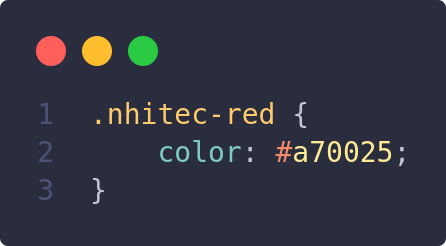
\includegraphics[width=0.4\linewidth]{figures-C1/css_nhitec_example.png}
    \caption{Exemple de classe \css{} pour la couleur \nhitec{}.}
    \label{fig:css-nhitec}
\end{figure}

\paragraph{Explication du code}
\begin{itemize}
    \item \verb|.nhitec-red| : sélecteur, nom de la classe \css{}.
    \item \verb|color| : propriété, en l'occurence la couleur.
    \item \verb|#a70025| : valeur, ici écrite en code héxadécimal.
\end{itemize}

\subsubsection[Pourquoi utiliser Tailwind?][fr.wikipedia.org/wiki/Tailwind\_CSS]{Pourquoi utiliser \tailwind{}?}
Créer un \css{} pour chaque propriété d'un composant peut prendre énormement de temps. C'est pour cela que de nombreux \textit{frameworks front-end\footnote{Le \textit{front-end, en opposition au back-end, désigne tout ce qui constitue l'interface visible par l'utilisateur (ex.: page web, images, etc\ldots}}.} existent afin d'amener de nombreuses \verb|class| et plugins \js{} prédéfinis. En l'occurrence, nous allons utiliser \tailwind{}, qui est un \textit{framework} utilisé pour construire des sites de manière \textit{responsive\footnote{\textit{Responsive} signifie que le site/composant adapte son rendu en fonction de la taille de l'écran, du format etc, ce qui est quand même très important.}} rapidement et facilement.

Pour plus de renseignementss et pour découvrir les fonctionnalités de \tailwind{}, rendez-vous sur \href{https://tailwindcss.com/docs}{Doc \tailwind{}}. Dans votre futur, vous utiliserez énormément de \verb|class| \tailwind. Il est donc important de se familiariser avec rapidement, par exemple en lisant la documentation des \verb|class| que vous ne connaissez pas, même si c'est fort déroutant au début afin que cela roule tout seul à moyen terme.

\subsubsection[Installation]{Installation}

Pour installer \tailwind{}, la version 12 de \laravel{} nous facilite grandement la tâche car le \textit{framework} est directement intégré lors d'une nouvelle création de projet. Il n'y a donc rien a faire.

Cependant, nous allons ajouter notre \css{} contenant la couleur de notre chère et tendre \textit{JE}. Pour l'instant, le dossier \texttt{resources/css} ne possède qu'un seul fichier \texttt{app.css} qui inclut la bibliothèque de \tailwind{}. Nous allons, dans ce même dossier, créer un fichier \texttt{nhitec.css} qui va accueillir notre couleur créée précédemment. Ajoutons-y le contenu de la figure \ref{fig:css-nhitec}. Pour que notre fichier \texttt{nhitec.css} soit accessible par nos différentes vues, nous allons l'inclure dans le fichier \texttt{resources/js/types/app.jsx} comme à la figure \ref{fig:include_css}

\begin{figure}[H]
    \centering
    % Première figure
    \begin{minipage}[b]{0.34\linewidth}
        \centering
        
\includegraphics[width=0.9\linewidth]{figures-C1/app.css_directory.png}
        \caption{Dossier contenant les fichiers \texttt{.css}}
        \label{fig:app.css_directory}
    \end{minipage}
    \hspace{0.04\linewidth}
    % Deuxième figure
    \begin{minipage}[b]{0.45\linewidth}
        \centering
        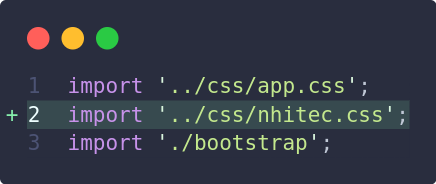
\includegraphics[width=0.9\linewidth]{figures-C1/include_css.png}
        \caption{\texttt{app.jsx}}
        \label{fig:include_css}
    \end{minipage}
\end{figure}





\subsubsection[Utilisation]{Utilisation} \label{sec:utilisation}

Comme expliqué plus haut, \tailwind{} nous fournit une multitude de \verb|class| que nous pouvons utiliser pour styliser nos \textit{tags} \html{}. Modifions donc nos pages \verb|About.jsx| et \verb|Index.jsx| comme aux \textsc{Figures~\ref{fig:about_bs}\&\ref{fig:index_bs}}.

\SaveVerb{about}|About.jsx|
\SaveVerb{index}|Index.jsx|
\begin{figure}[!ht]
    \centering
    \begin{minipage}{0.45\textwidth}
         \centering
         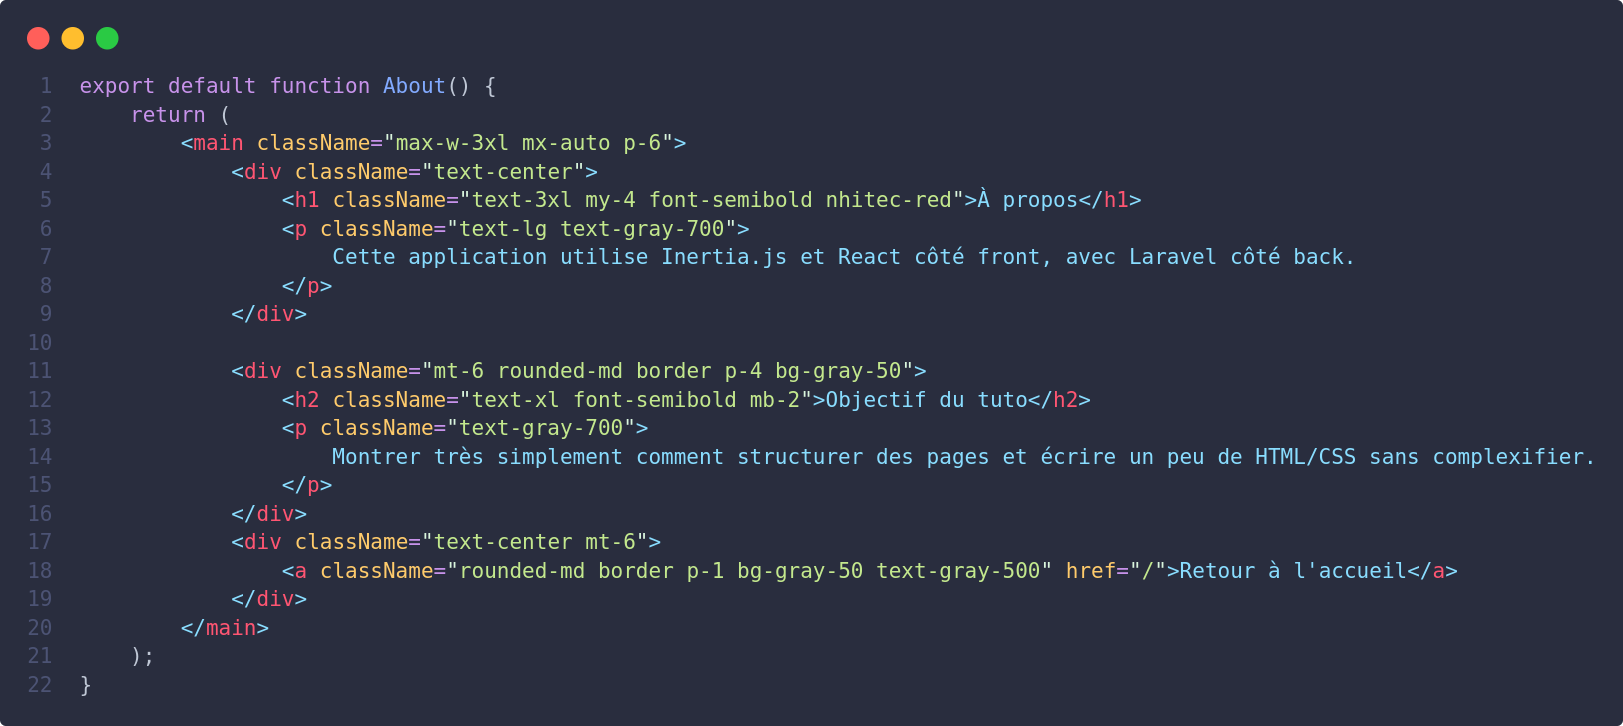
\includegraphics[width=\textwidth]{figures-C1/about.jsx.png}
         \caption{\protect\UseVerb{about}\label{fig:about_bs}}
    \end{minipage}
    \begin{minipage}{0.53\textwidth}
         \centering
         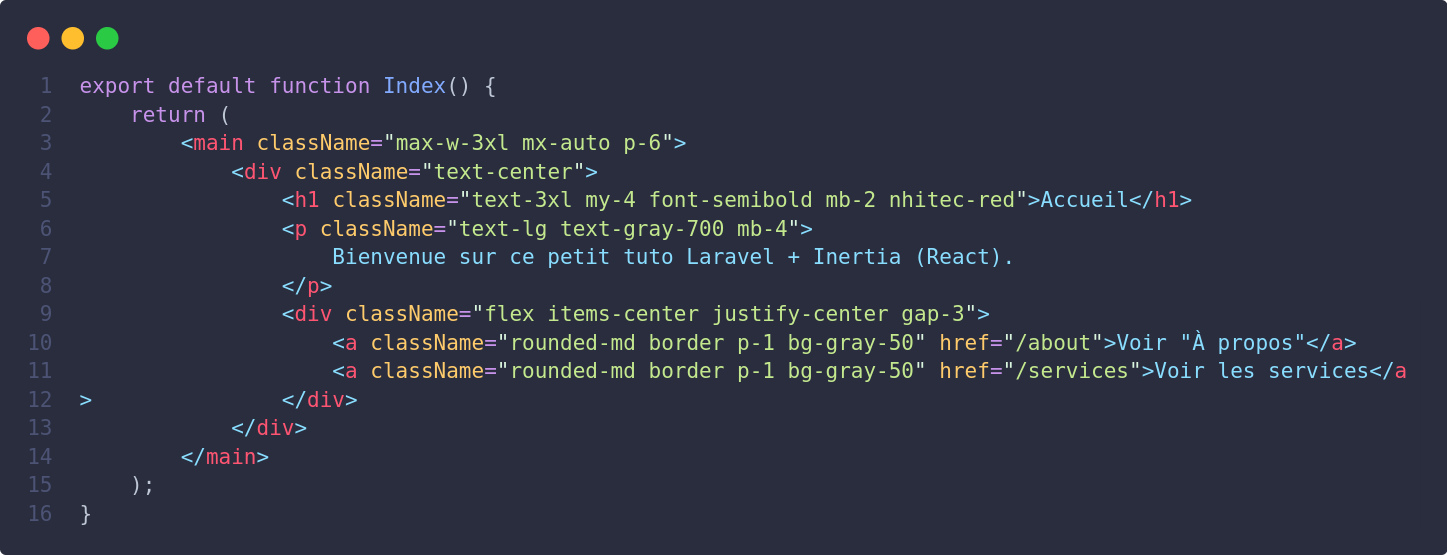
\includegraphics[width=\textwidth]{figures-C1/index.jsx.png}
         \caption{\protect\UseVerb{index}\label{fig:index_bs}}
    \end{minipage}
\end{figure}

\begin{wrapfigure}{r}{0.35\textwidth}
    \vspace{-0.5cm}
    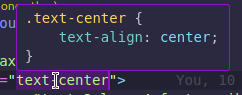
\includegraphics[width=0.35\textwidth]{figures-C1/tailwind_intellisense.png}
\end{wrapfigure}
Par exemple, dans la \textsc{Figure~\ref{fig:about_bs}}, \verb|className="text-center"| assigne la classe \verb|text-center| à l'élément. Astuce : En passant la souris sur la classe \tailwind{}, vous verrez apparaître la vraie classe \css{}\footnote{Grâce à une extension incluse dans le pack N-HiTec - Op\&Ex.} permettant de centrer un élément dans son conteneur.



Pour la page des services, nous allons introduire une nouvelle mécanique : l'\textbf{affichage dynamique} c-à-d passer des données du back-end vers le front-end. \footnote{C'est comme ça que votre nom d'utilisateur est affiché sur les réseaux sociaux. Le nom d'utilisateur est récolté dans la base de données et envoyé au front-end qui l'affiche sur l'interface utilisateur.} Pour le moment, nous n'allons pas encore nous embêter avec la base de données, nous allons simplement voir comment la mécanique de base fonctionne. Rappelez-vous de la \texttt{Section~\ref{sec:fonctionnement&philosophie}}, ce sont les \controllers{} qui s'occupent de manipuler les données avant d'afficher une page. Dès lors, c'est dans la fonction \verb|services()| de \verb|PagesController.php| que nous allons ajouter des choses: \verb|$titlefromcontroller| et \verb|$services| sont 2 variables, et nous les passons à la page par l'intermédiaire du \verb|[]|. Ensuite, nous pouvons utiliser les variables \verb|title| et \verb|services| dans la page concernée.

\begin{figure}[h]
    \centering
    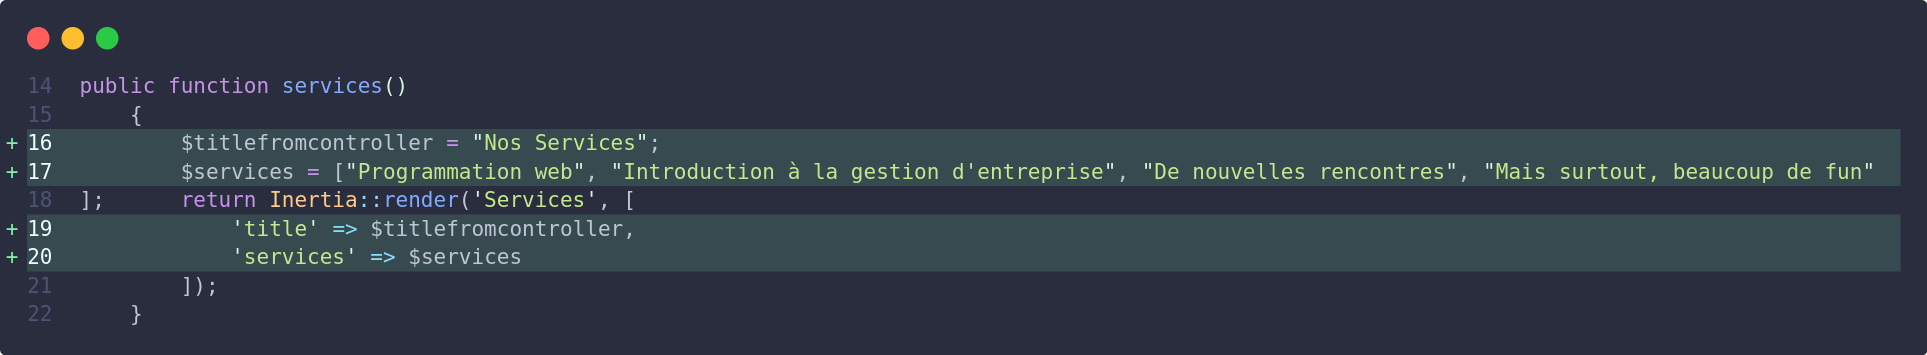
\includegraphics[width=\textwidth]{figures-C1/services_update.png}
    \caption{\texttt{PagesController.services}}
\end{figure}

\newpage

\begin{figure}
    \centering
    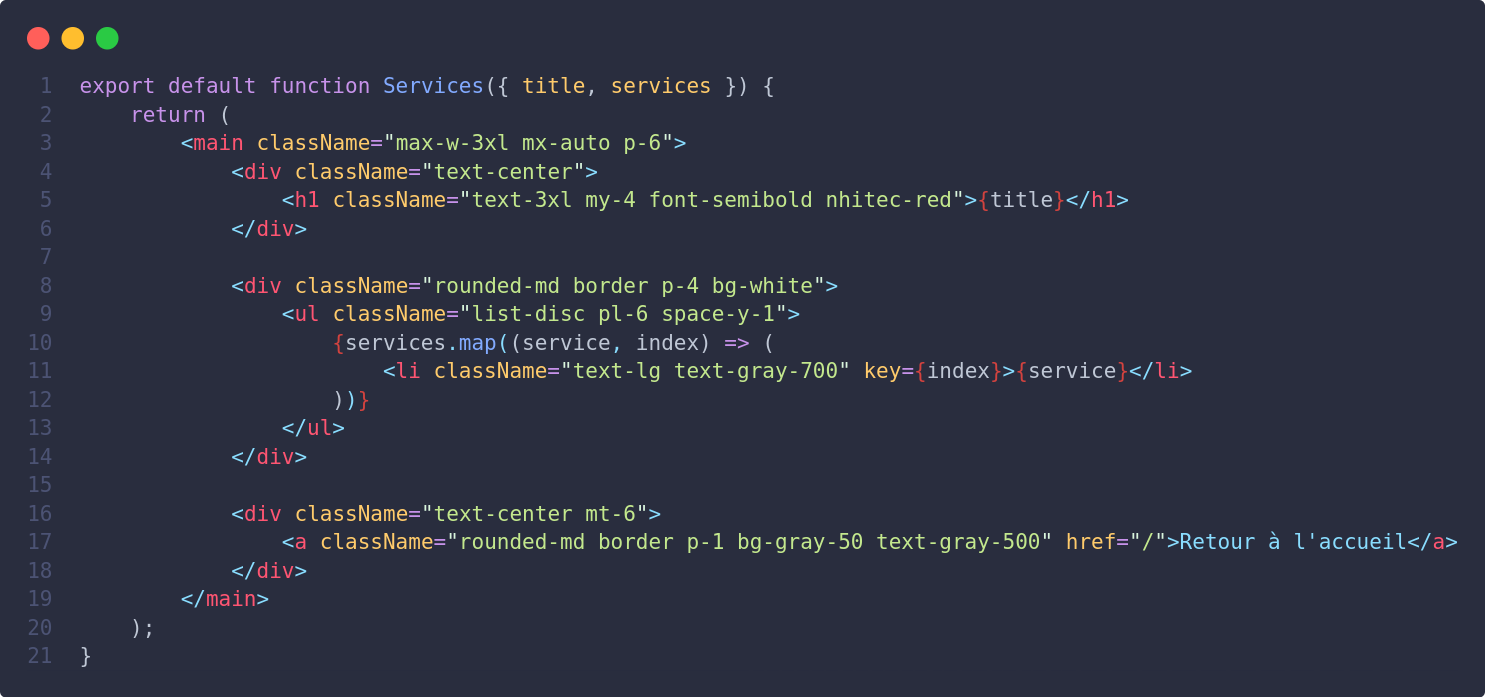
\includegraphics[width=0.5\textwidth]{figures-C1/services.jsx.png}
    \caption{\texttt{Services.jsx}}
\end{figure}

Qu'est-ce que c'est que tout ça? Décomposons tout cela.

 Dans la \texttt{Section~\ref{sec:welcome!}} nous avons pris connaissance des avantages du format \verb|.jsx|. Celui-ci nous apporte les commandes \verb|{}| \footnote{Cette commande agit comme un \verb|printf()| en C. Elle permet d'afficher le contenu de la variable en argument.} et \verb|.map| \footnote{Boucle \verb|for| classique, pour itérer sur un tableau.}.

\begin{minipage}{\textwidth}
De plus, nous découvrons ici trois nouveaux tags \html{}:

\begin{enumerate}
    \item \verb|<a>| est un tag permettant la création d'un lien vers une autre URL, que l'on place dans l'attribut \verb|href|. Au lieu de tapez l'URL d'une \route{}, \inertia{} nous permet d'optimiser l'écriture en utilisant la commande \verb|route('nomdelaroute')| afin d'obtenir l'URL en question.~\verb|{...}| permet ensuite de l'afficher dans le \verb|href|.
    \item \verb|<ul>| est un tag signifiant la création d'une liste.
    \item \verb|<li>| représente un élément d'une liste.
\end{enumerate}
\end{minipage}


Et voilà! Maintenant, il suffit de taper \verb|npm run dev|\footnote{Cette commande permet de compiler le \css{} et \js{} en créant un mini serveur localement. Cette commande utilisée lors du \underline{DEVELOPPEMENT DU SITE} permet d'appliquer les modifications apportées à des fichiers rapidement sans devoir refresh la page. Pour compiler tout ça en production, il faut utiliser \verb|npm run build|.}(si ce n'était pas déjà fait) pour admirer le résultat \footnote{L'url à entrer dans la barre de recherche dépend de la variable \texttt{APP\_URL} se trouvant dans le \texttt{.env}.} (voir \textsc{Figure~\ref{fig:3pages}}). C'est déjà vachement mieux, non?

\begin{figure}[!h]
    \begin{subfigure}[c]{0.60\textwidth}
        \fbox{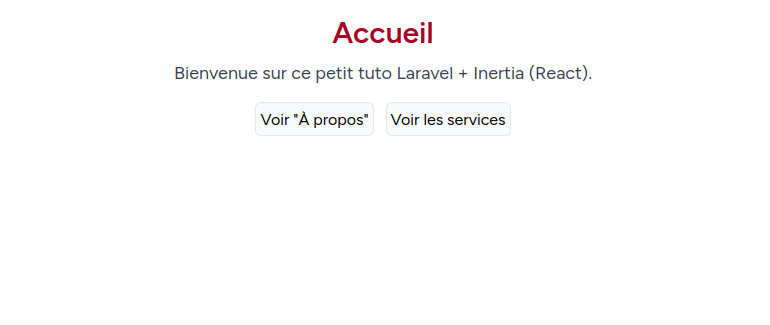
\includegraphics[width=\textwidth]{figures-C1/index_page.png}}
    \end{subfigure}\hfill
    \begin{subfigure}[c]{0.35\textwidth}
        \caption{\url{http://tutolaravel/}} 
    \end{subfigure}
    \begin{subfigure}[c]{0.60\textwidth}
        \fbox{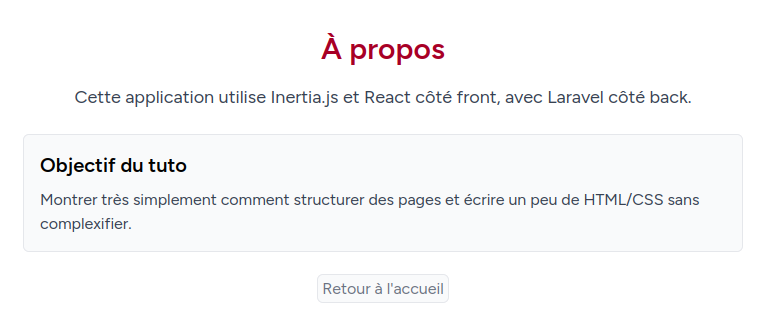
\includegraphics[width=\textwidth]{figures-C1/about_page.png}}
    \end{subfigure}\hfill
    \begin{subfigure}[c]{0.35\textwidth}
        \caption{\url{http://tutolaravel/about}}
    \end{subfigure}
    \begin{subfigure}[c]{0.60\textwidth}
        \fbox{
\includegraphics[width=\textwidth]{figures-C1/services_page.png}}
    \end{subfigure}\hfill
    \begin{subfigure}[c]{0.35\textwidth}
        \caption{\url{http://tutolaravel/services}} 
    \end{subfigure}
    \caption{3 pages créées jusqu'à présent et stylisées avec \tailwind{}.}
    \label{fig:3pages}
\end{figure}

C'est bien beau, mais jusque ici le seul moyen de naviguer entre les pages est de rentrer leur URL ou revenir à l'accueil, ce qui n'est ma foi pas très pratique. Remédions à cela avant de passer à la suite.

\subsubsection[Navbar]{Navbar}\label{sec:navbar}



Comme son nom l'indique, elle sert à naviguer entre les pages. Cependant, c'est un gros morceau qui utilise beaucoup de \verb|class| \tailwind{}, donc il va falloir s'accrocher.

Heureusement pour nous, \react{} inclut une bibliothèque de composants prêts à l'emploi \footnote{Ceux-ci se trouvent dans \texttt{resources/js/Components}.}. Dans notre exemple, nous allons utiliser \texttt{ResponsiveNavLink.jsx}.

D'abord, dans le dossier \verb|resources/js/Layouts|, créez un fichier \verb|AppLayout.jsx|. Remplissez ce fichier avec le contenu de la \textsc{Figure~\ref{fig:navbar}}.

\begin{wrapfigure}[7]{R}{0.43\textwidth}
    \vspace{-1.2cm}
    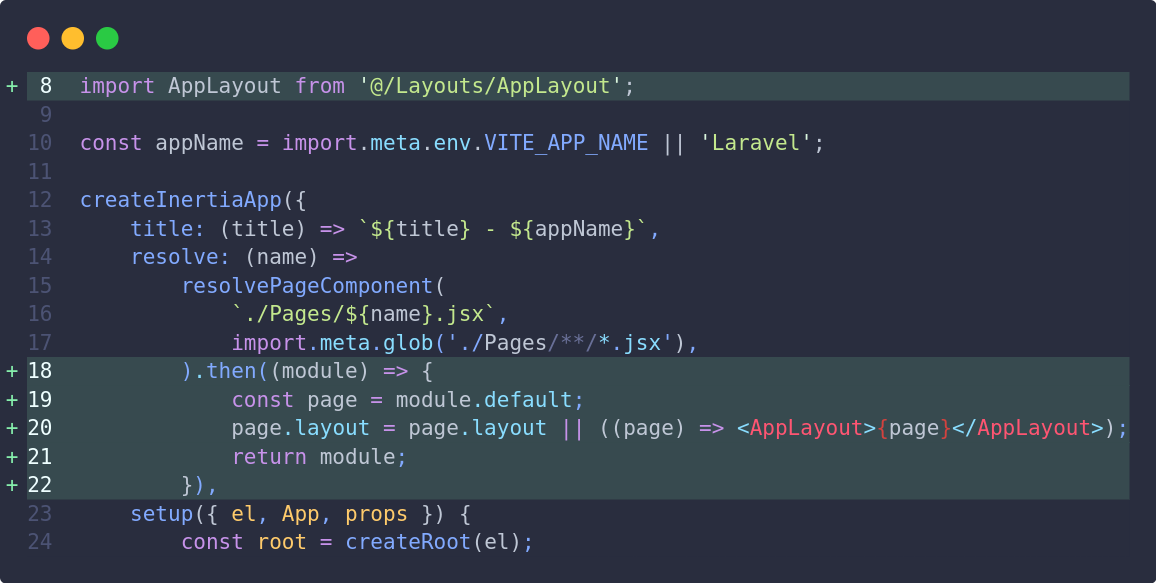
\includegraphics[width=0.5\textwidth]{figures-C1/app.jsx.png}
\end{wrapfigure}

\enlargethispage{2\baselineskip}

Ensuite, il faut ajouter notre \textit{navbar} à notre \textit{layout} afin qu'elle apparaisse sur toutes nos pages. Pour ce faire, rien de plus simple. Ajoutez ce bout de code dans \texttt{resources/js/app.tsx}.

\begin{figure}[!h]
    \centering
    \begin{minipage}{0.7\textwidth}
         \centering
         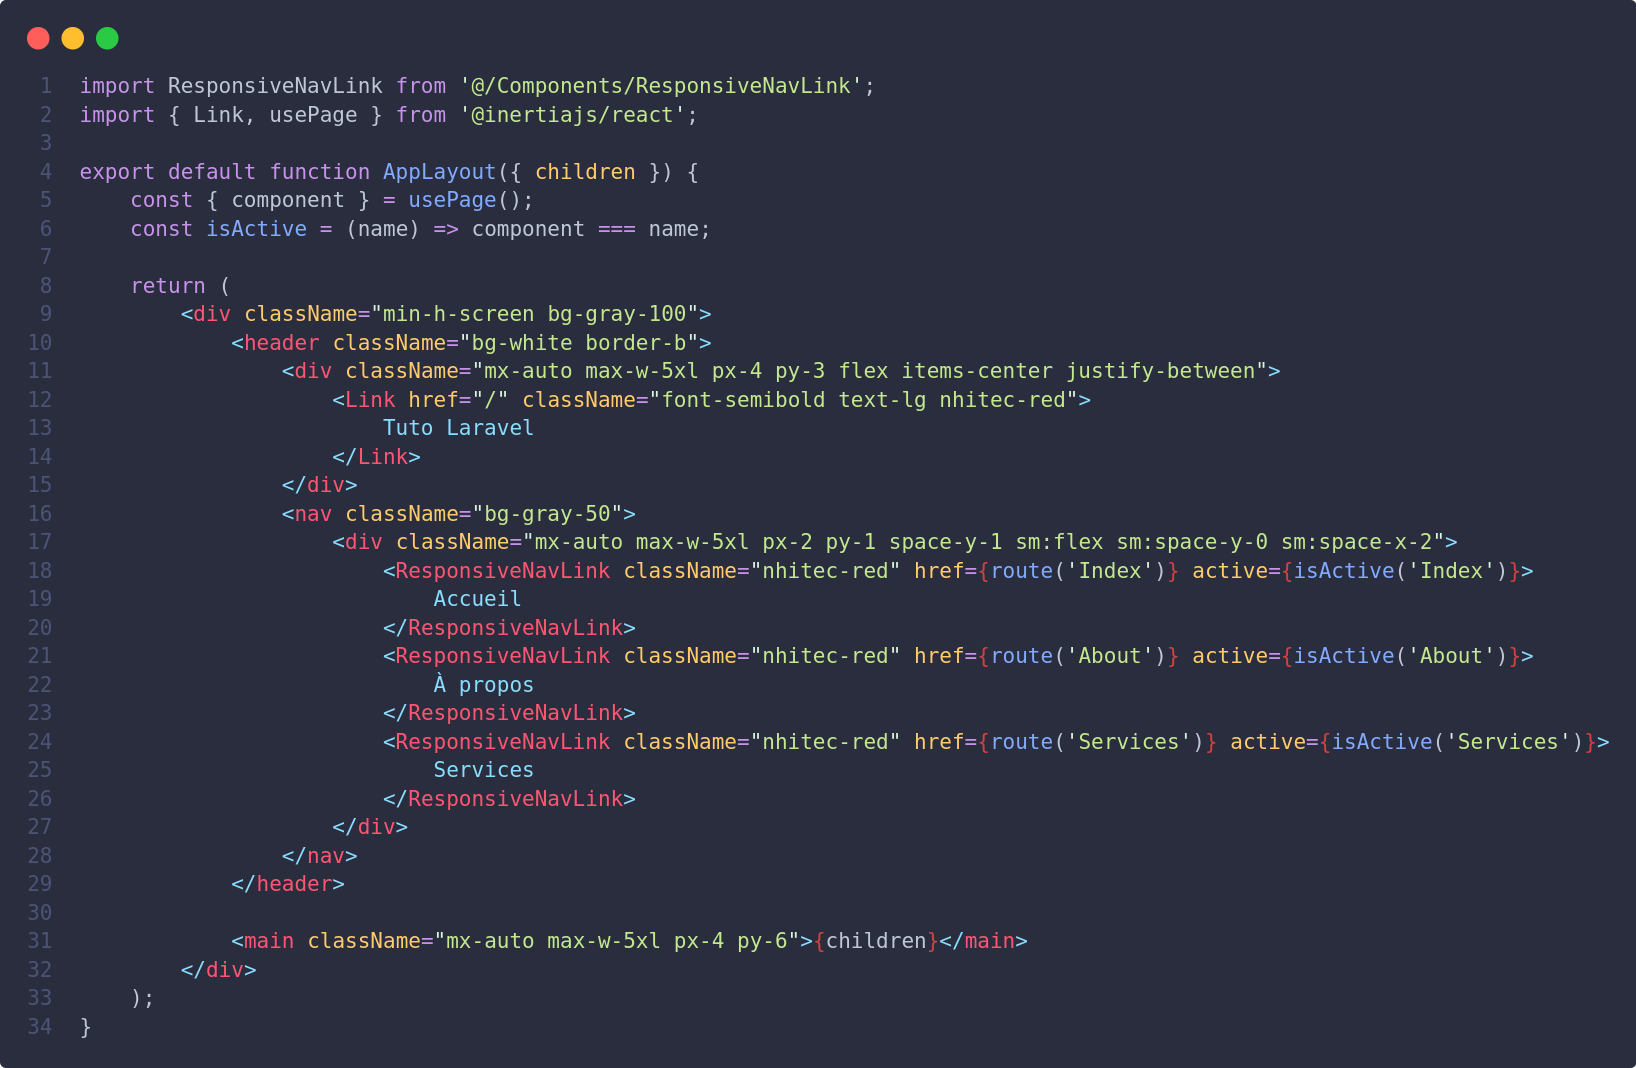
\includegraphics[width=.9\textwidth]{figures-C1/AppLayout.jsx.png}
         \caption{\texttt{AppLayout.jsx}\label{fig:navbar}}
    \end{minipage}
    \begin{minipage}{0.28\textwidth}
        \vspace{1cm}
         \centering
         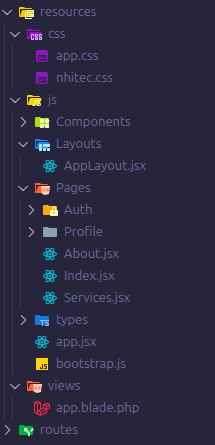
\includegraphics[width=0.77\textwidth]{figures-C1/repo_directory.png}
         \caption{\newline Structure du projet}
    \end{minipage}
\end{figure}

Pour le reste, je vous invite à lire ce que font chaque \verb|class| et de jeter un œil sur \href{https://getTailwind.com/docs/5.3/components/navbar/}{la doc \tailwind{} sur les navbars}. Bien que ça soit indigeste lors d'une première lecture, ça l'est beaucoup moins que si nous devions analyser les \verb|class| une par une \ldots.

Néanmoins, il reste un point important à aborder : le \textit{responsive design} ou \textit{design adaptatif}, c'est le fait de modifier la page web en fonction de la taille de la fenêtre pour convenir à tous les supports.

\newpage

\begin{figure}[!h]
    \centering
        \fbox{
\includegraphics[width=\textwidth]{figures-C1/navbar_big_size.png}}
        \caption{Navbar sur un écran de largeur $>640\mathrm{px}$}
\end{figure}
\begin{figure}[!h]
        \centering
        \fbox{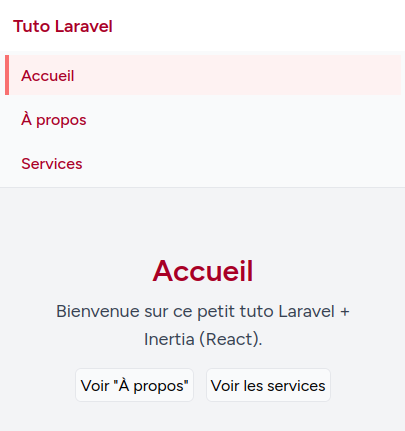
\includegraphics[width=0.2\textwidth]{figures-C1/navbar_phone_size.png}}
        \caption[La couleur rouge est obtenue en remplaçant les mentions \texttt{indigo} par \texttt{red} dans \texttt{ResponsiveNavLink.tsx}]{Navbar vue depuis un téléphone (largeur $<640\mathrm{px}$) \footnotemark}
\end{figure}
\footnotetext{La couleur rouge est obtenue en remplaçant les \texttt{class} \css{} \texttt{indigo} par \texttt{red} dans \texttt{ResponsiveNavLink.tsx}.}

\newpage
